\chapter{Results}
\label{chap:results}

\section{Final-answer benchmark}

The lexical benchmark establishes the outcome pattern before intermediate states are considered. On the harder MuSiQue subset, the frozen SAS achieves final normalised accuracy of 0.560 at the 1,000-token budget and 0.525 at 2,000. Debate is the strongest MAS in this condition, at 0.510 and 0.535 respectively. Sequential is substantially lower, at 0.335 and 0.340. Fine-tuning does not reverse the broad ranking: at 1,000 tokens the \texttt{v3b} SAS scores 0.545, Debate 0.505, and Sequential 0.380.

\begin{table}[htbp]
  \centering
  \caption[MuSiQue final lexical accuracy]{MuSiQue final normalised lexical accuracy by model, architecture, and thinking-token budget ($n=200$ per cell).}
  \label{tab:musique-lexical}
  \begin{tabular}{@{}llrr@{}}
    \toprule
    Model & System & 1,000 & 2,000 \\
    \midrule
    Frozen & SAS & \textbf{0.560} & 0.525 \\
           & Debate & 0.510 & \textbf{0.535} \\
           & Ensemble & 0.520 & 0.505 \\
           & Parallel Roles & 0.425 & 0.390 \\
           & Sequential & 0.335 & 0.340 \\
           & Subtask Parallel & 0.425 & 0.425 \\
    \addlinespace
    v3b & SAS & \textbf{0.545} & \textbf{0.530} \\
        & Debate & 0.505 & \textbf{0.530} \\
        & Ensemble & 0.515 & 0.510 \\
        & Parallel Roles & 0.415 & 0.445 \\
        & Sequential & 0.380 & 0.340 \\
        & Subtask Parallel & 0.410 & 0.390 \\
    \bottomrule
  \end{tabular}
\end{table}

On 2WikiMultiHopQA, absolute performance is much higher. In the frozen condition, Debate reaches 0.935 and 0.930 at the two budgets, compared with SAS at 0.860 and 0.845. This is an important counterexample to any universal statement that a single agent always wins: an MAS can outperform the SAS on a particular dataset and configuration. The dissertation's claim is narrower. Multi-agent decomposition often increases candidate availability, but that gain is inconsistent and is partly lost at later coordination stages. The relative behaviour also depends on dataset difficulty, answer distribution, and architecture.

The lexical results alone cannot show whether Debate's stronger 2Wiki score is caused by better exploration or better selection, nor why Ensemble and Parallel Roles underperform despite producing several candidates. The semantic analysis addresses that question.

\section{Semantic discovery, oracle coverage, and aggregation regret}

The full-trace Mistral screen indicates that independent-candidate architectures frequently make the correct answer available before the final decision. For frozen MuSiQue at 1,000 tokens, Debate has final semantic accuracy 0.720 and candidate-oracle accuracy 0.845, giving aggregation regret of 0.125. Ensemble has final accuracy 0.660 and oracle accuracy 0.960, a regret of 0.300. Parallel Roles is more extreme: final accuracy 0.600 versus oracle 0.915, a regret of 0.315. These gaps are too large to describe as candidate-generation failure alone.

\begin{figure}[htbp]
  \centering
  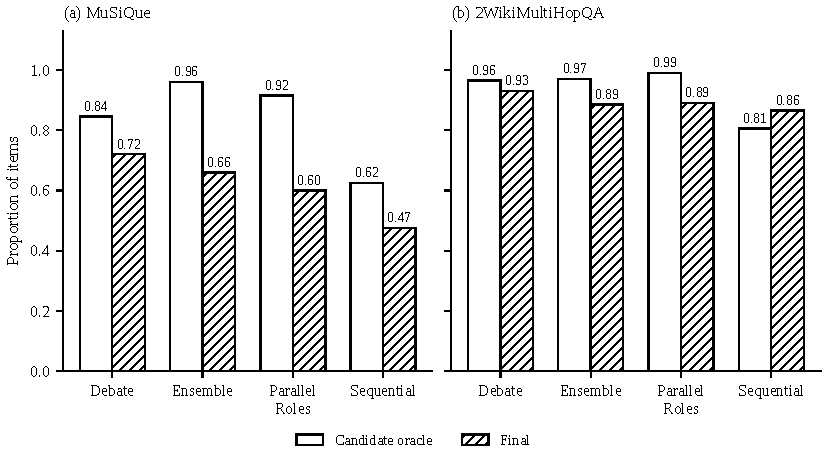
\includegraphics[width=0.94\textwidth]{figures/semantic_oracle_final.pdf}
  \caption[Candidate-oracle and final semantic accuracy]{Machine-screened candidate-oracle and final semantic accuracy for the frozen model at the 1,000-token budget. Higher oracle than final accuracy indicates that a correct candidate was available but not selected. Subtask Parallel is omitted because its worker outputs are partial findings rather than full-answer candidates.}
  \label{fig:oracle-final}
\end{figure}

\Cref{fig:oracle-final} shows that the gap is dataset dependent. On frozen 2Wiki at 1,000 tokens, Debate's final accuracy is 0.930 and its oracle accuracy 0.965, a regret of only 0.035. Ensemble and Parallel Roles still show positive regret, at 0.085 and 0.100. Easier questions allow both candidates and aggregators to be more reliable; on MuSiQue, candidate diversity increases without a comparable increase in final decision quality.

The semantic diversity statistic supports this interpretation. Frozen MuSiQue Parallel Roles has diversity rate 0.650 and a mean of four distinct candidate texts, while its final semantic accuracy is only 0.600. Ensemble has mean 3.835 distinct candidates and final accuracy 0.660. Diversity is therefore a resource, not an outcome. It creates selection opportunities and selection risk simultaneously.

Sequential behaves differently. On frozen MuSiQue at 1,000 tokens, candidate-oracle accuracy is 0.625 and final accuracy is 0.475, but the meaning of a candidate is tied to the last worker rather than independent full answers. On 2Wiki, final accuracy can exceed the worker oracle summary (0.865 final versus 0.805 oracle at 1,000), producing negative regret. This is consistent with an aggregator synthesising partial or implicit findings into a correct final response. Negative regret does not imply perfect preservation; it indicates that the final stage sometimes creates answer-equivalent content not credited at the designated source candidates.

\section{Machine-screened failure localisation}

Across 8,000 MAS item-configurations, the first-error-stage screen classifies 5,876 trajectories as finally correct under the machine label and 2,124 as terminal failures. Among all configurations, 946 first fail at proposal or initial worker output, 73 at Debate revision, 75 within the Sequential worker chain, 173 at the Debate final picker, and 857 at final aggregation. The last category includes Ensemble, Parallel Roles, Sequential, and Subtask Parallel and is the largest localised failure point.

\begin{table}[htbp]
  \centering
  \caption[Machine-screened first-error locations]{Machine-screened first-error location over 8,000 MAS configurations. Counts are descriptive screening estimates, not human-validated totals.}
  \label{tab:first-error}
  \small
  \setlength{\tabcolsep}{4pt}
  \begin{tabular}{@{}lrrrrrr@{}}
    \toprule
    System & Proposal & Revision & Worker chain & Picker & Aggregator & Final correct \\
    \midrule
    Debate & 77 & 73 & 0 & 173 & 0 & 1,277 \\
    Ensemble & 66 & 0 & 0 & 0 & 316 & 1,218 \\
    Parallel Roles & 77 & 0 & 0 & 0 & 336 & 1,187 \\
    Sequential & 376 & 0 & 75 & 0 & 94 & 1,055 \\
    Subtask Parallel & 350 & 0 & 0 & 0 & 111 & 1,139 \\
    \midrule
    All & 946 & 73 & 75 & 173 & 857 & 5,876 \\
    \bottomrule
  \end{tabular}
\end{table}

Within Debate, the screen counts 278 harmful proposal-to-revision flips and 169 beneficial flips. A targeted human sensitivity audit exactly confirmed 13 of 24 resolved sampled harmful flips and 11 of 25 beneficial flips. A descriptive projection retained the direction harmful greater than beneficial, but the modest confirmation rates mean the raw full-trace counts cannot be presented as exact semantic totals. Similarly, the machine screen identifies 142 Sequential items where the worker chain ends wrong after earlier discovery and 94 in which the aggregator loses a correct last-worker answer. Only 8 of 25 sampled machine-labelled Sequential \ctow{} transitions were exactly confirmed in the targeted audit, mainly because the judge over-called source correctness.

These results justify, but do not substitute for, the final human audit. They locate picker and aggregator boundaries as high-value targets and reveal which machine strata require manual review.

\section{Human audit reliability}

The 20 hidden repeated stages produced exact agreement of 20/20 on both Discovery and Endorsement, with $\kappa=1.000$ and bootstrap intervals $[1.000,1.000]$. This shows perfect repeatability for the inserted records. It does not show independent inter-annotator validity because the same annotator labelled both blind copies.

Against the frozen Mistral stage labels, human agreement is 330/400 (82.5\%) for Discovery and 322/400 (80.5\%) for Endorsement. Cohen's kappa is 0.632 (95\% bootstrap CI $[0.557,0.705]$) for Discovery and 0.617 ($[0.541,0.691]$) for Endorsement. These are substantial enough for a broad screen, but the 70 Discovery disagreements and 78 Endorsement disagreements are not negligible in a transition analysis.

\begin{table}[htbp]
  \centering
  \caption[Human audit reliability]{Human audit reliability. Human-machine agreement uses 400 non-repeat stage records; repeat agreement uses 20 hidden pairs.}
  \label{tab:agreement}
  \begin{tabular}{@{}llrrl@{}}
    \toprule
    Comparison & Axis & Exact agreement & $\kappa$ & 95\% CI \\
    \midrule
    Hidden repeat & Discovery & 20/20 (100.0\%) & 1.000 & [1.000, 1.000] \\
    Hidden repeat & Endorsement & 20/20 (100.0\%) & 1.000 & [1.000, 1.000] \\
    Human--Mistral & Discovery & 330/400 (82.5\%) & 0.632 & [0.557, 0.705] \\
    Human--Mistral & Endorsement & 322/400 (80.5\%) & 0.617 & [0.541, 0.691] \\
    \bottomrule
  \end{tabular}
\end{table}

Across all 420 annotated rows, the 14 cases with Discovery \correct{} and Endorsement \wrong{} demonstrate why a single semantic-correctness label is insufficient. The stage contains the answer but does not support the system selecting it. A presence-oriented judge is likely to over-credit precisely these cases.

\section{Human transition estimates}

The raw audited item transitions were sharply different by architecture. Debate contained 35 \correct$\rightarrow$\correct, 19 \ctow, zero \wtoc, 25 \wrong$\rightarrow$\wrong, and one \uncertain$\rightarrow$\wrong item. Sequential contained 40 \correct$\rightarrow$\correct, four \ctow, six \wtoc, 29 \wrong$\rightarrow$\wrong, and one \uncertain$\rightarrow$\wrong item. Because rare machine-defined transition strata were oversampled, the weighted rates rather than these raw proportions are used for population interpretation.

\begin{figure}[htbp]
  \centering
  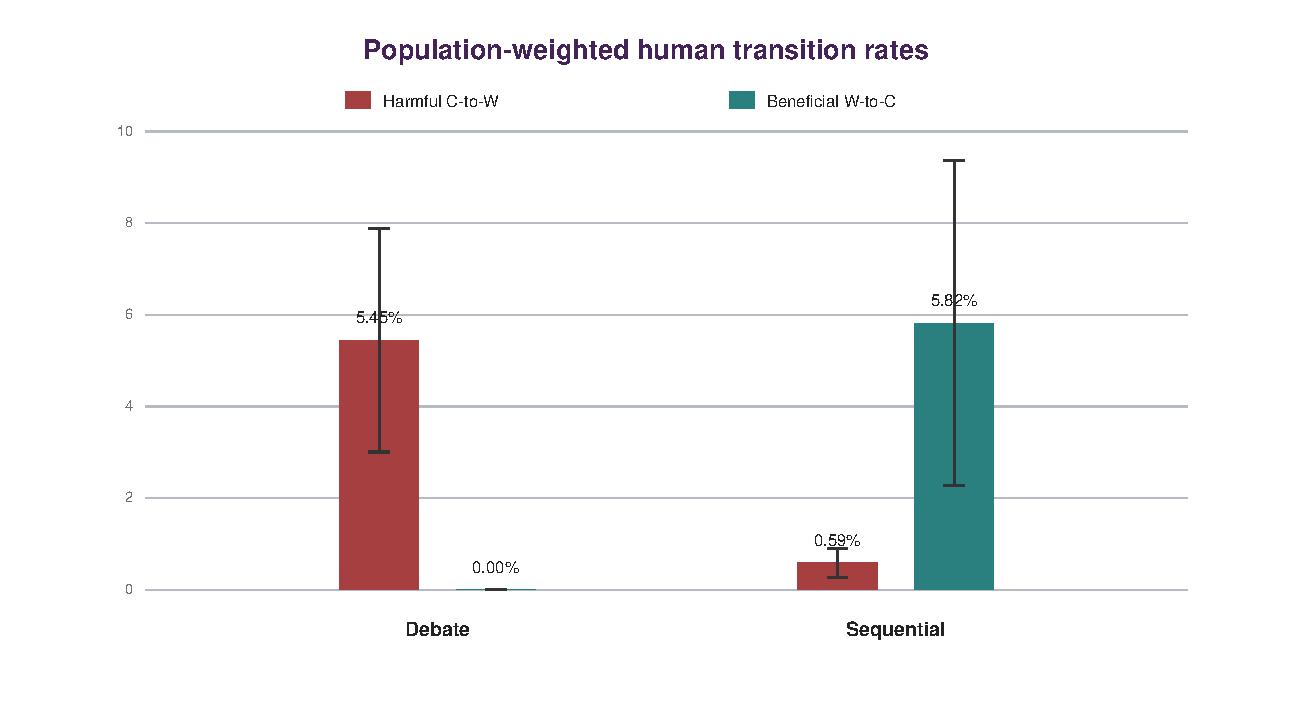
\includegraphics[width=0.88\textwidth]{figures/human_transition_rates.pdf}
  \caption[Population-weighted human transition rates]{Population-weighted human Endorsement transition rates under the primary \uncertain$\rightarrow$\wrong{} rule. Error bars are approximate 95\% finite-population stratified intervals.}
  \label{fig:human-transitions}
\end{figure}

Debate's weighted harmful \ctow{} rate is 5.45\% (approximate 95\% CI $[3.01,7.89]$), compared with 0.59\% for Sequential ($[0.27,0.90]$). The Debate-minus-Sequential difference is 4.86 percentage points ($[2.41,7.32]$). The beneficial \wtoc{} pattern is reversed: 0.00\% for Debate and 5.82\% for Sequential ($[2.28,9.37]$). The one machine-defined Debate beneficial picker event in the sampling census was human \correct$\rightarrow$\correct after unblinding, so no audited Debate wrong source was corrected by the picker.

Using source Discovery rather than source Endorsement gives a weighted probability that a discovered answer is not endorsed in the final output of 7.06\% for Debate and 3.96\% for Sequential. This second measure captures loss between informational presence and decision, including cases where a correct answer was discovered without being cleanly endorsed at the source.

The uncertain-label sensitivity analysis does not reverse the main harmful-rate ordering. Under \uncertain$\rightarrow$\wrong, exclusion of uncertain-bearing items, and \uncertain$\rightarrow$\correct, Debate's harmful rate is 5.45\%, 5.51\%, and 6.58\%, while Sequential's is 0.59\%, 0.60\%, and 2.20\%. The absolute Sequential estimate is more sensitive because one uncertain case has greater influence in a low-rate architecture, but Debate remains higher under every rule.

\section{Budget effects}

The matched budget analysis provides no evidence that doubling the nominal thinking allowance improves aggregate MAS outcomes. Across 3,997 resolved discovery pairs, semantic discovery falls from 0.8419 at 1,000 tokens to 0.8284 at 2,000. There are 138 wrong-to-correct changes but 192 correct-to-wrong changes; the exact McNemar $p$-value is 0.0035. Across all 4,000 final pairs, semantic final accuracy falls from 0.7408 to 0.7282, with 241 wrong-to-correct and 291 correct-to-wrong changes ($p=0.0335$). Mean wall time rises by 4.83 seconds and mean realised thinking increases by approximately 495 tokens.

\begin{figure}[htbp]
  \centering
  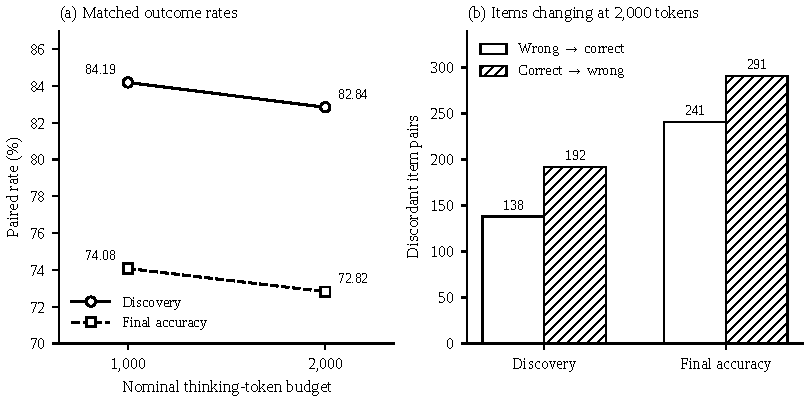
\includegraphics[width=0.92\textwidth]{figures/budget_tradeoff.pdf}
  \caption[Matched budget outcomes]{Matched aggregate outcomes at 1,000 and 2,000 nominal thinking tokens. The larger budget increases mean wall time while reducing machine-screened discovery and final semantic accuracy.}
  \label{fig:budget}
\end{figure}

The architecture-level results are heterogeneous. Debate final accuracy changes from 0.8113 to 0.7850 ($p=0.106$), Ensemble from 0.7725 to 0.7500 ($p=0.066$), Parallel Roles from 0.7425 to 0.7412 ($p=1.000$), Sequential from 0.6650 to 0.6538 ($p=0.426$), and Subtask Parallel from 0.7125 to 0.7113 ($p=1.000$). None of these individual final-accuracy comparisons reaches the conventional 0.05 level. The aggregate decline is produced by many small, mostly non-improving changes across cells rather than one architecture collapsing.

Latency increases in every system. Debate mean wall time rises from 15.38 to 22.92 seconds; Ensemble from 7.57 to 10.88; Parallel Roles from 9.94 to 14.79; Sequential from 17.89 to 22.58; and Subtask Parallel from 11.66 to 15.40. Parallel systems have shorter critical paths, but this should not be confused with lower total device work.

\section{Resource associations and truncation}

Within matched design strata, observations above the median wall time have lower odds of discovery (adjusted OR 0.657, 95\% CI $[0.574,0.753]$) and higher odds of dropping the answer after discovery (OR 1.768, $[1.529,2.044]$). Above-median realised thinking tokens show the same direction: OR 0.529 ($[0.456,0.613]$) for discovery and OR 2.679 ($[2.153,3.334]$) for post-discovery drop.

\begin{figure}[htbp]
  \centering
  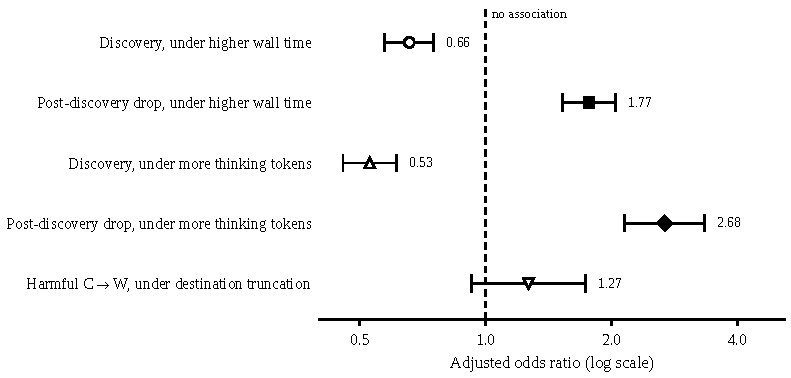
\includegraphics[width=0.90\textwidth]{figures/resource_associations.pdf}
  \caption[Resource exposure and semantic outcomes]{Adjusted observational odds ratios for resource exposure and semantic outcomes. Values below one favour the unexposed group for the named outcome; intervals are 95\% confidence intervals. These associations are not causal effects.}
  \label{fig:resources}
\end{figure}

These results do not mean that fewer tokens causally improve reasoning. Difficult or unstable items may elicit longer trajectories, and repeated unsuccessful revisions may consume both time and tokens. They do show that realised compute is not a valid proxy for productive reasoning in this experiment.

Destination-stage truncation has OR 1.268 for a \ctow{} transition conditional on a correct machine-labelled source, with 95\% CI $[0.926,1.736]$ and $p=0.139$. The interval includes one, so the data do not establish a truncation effect. Furthermore, the targeted human audit found lower exact machine-human transition agreement for truncated destinations (0.412) than for non-truncated destinations (0.604). Truncation is thus both a plausible failure mechanism and a condition under which the automated judge is less dependable; the present evidence is insufficient to make a causal claim.

\section{Answers to the research questions}

For RQ1, MAS architectures often have high candidate discovery but do not consistently convert it into final performance under matched budgets. The result varies by dataset, with Debate outperforming SAS on frozen 2Wiki but not establishing a general advantage on MuSiQue. For RQ2, the human audit identifies the final picker as a net loss point for Debate and the final aggregator as a net recovery point for some Sequential items. For RQ3, the 2,000-token setting increases latency and realised tokens but reduces aggregate discovery and final semantic accuracy. The resource associations reinforce the conclusion that additional observed computation is correlated with, rather than protective against, unstable trajectories in these runs.
